\chapter{Ergebnisse}
In diesem Kapitel werden zunächst
Eigenschaften der Floquet-Theorie an dem Modell überprüft.
Des Weiteren wird die zeitliche Entwicklung
eines Zustandes durch den
Floquet-Formalismus mit der numerischen Lösung der
Schrödingergleichung verglichen. Es wird jeweils ein gemitteleter Strom berechnet und
ebenfalls verglichen.
Zum Ende soll das System auf zwei Elektronen erweitert werden und ebenso ein Strom berechnet werden.
In den folgenden Rechnungen wird der Sprungterm $J=1$ gesetzt und  alle Ergebnisse in Einheiten von J angegeben.
Desweitern wird in Atomaren Einheiten gerechnet folglich gilt
\begin{align}
   \symup{e}=\hbar=\text{m}_\symup{e}=1.
\end{align}
\section{Frequenzabbhängigkeit der Quasienergien}
Zu Begin werden die Eigenwerte $\epsilon_{\alpha n}$ für eine Matrix $\mathcal{H}_\mathrm{F}$ mit eine Größe der Matrix $n=1$
bei konstanter lokaler Energie $a=??$ und E-Feldstärke $E_0=??$ für unterschiedliche Frequenz berechnet.
Hier mit soll die Frequenzabhängigkeit \eqref{eqn:epsilon_n} der Eigenwerte der Matrix $\mathcal{H}_\mathrm{F}$
überprüft werden.
Die Eigenwerte $\epsilon_\alpha$ so wie die Eigenwerte $E_{\alpha n}$ des zeitunabhängiges System
die nach der Formel \eqref{eqn:epsilon_n}
sind in der Abbildung \ref{fig:epsilon_f} dargestellt.
\begin{figure}
   \centering
   \includegraphics[width=0.7\textwidth]{C:/Users/daghe/Desktop/Uni/Bachelorarbeit/Freqenzen_kontinuierlich/Plots/Plot_fur_a=2.0_E=0.1.pdf}
   \caption{Eigenwerte $\epsilon_{\alpha n}$ der Matrix $\mathcal{H}_\mathrm{F}$ für $a=??$ und $E_0=??$ in Abhängigkeit von der Frequnez $\omega$.
    Die schwarzen Linien sind die nach der Gleichung \eqref{eqn:epsilon_n} berechneten Eigenwerte für das zeitunabhängige System}
   \label{fig:epsilon_f}
\end{figure}
Aus der Abbildung \ref{fig:epsilon_f} kann entnommen werden, dass die Eigenwerte $\epsilon_{\alpha n}$
(ADD)
\section{Brillouin-Zone der Quasienergien}
Nun sollen versucht werden die Eigenwerte wie in \ref{sec:flotheo} berschrieben in einer Art Brillouin-Zone darzugestellen.
Dafür werden Quasieenergien bei eine konstante Frequenz $\omega=??$ und lokale Energie $a=??$ in Abhängigkeit der
Amplitude $E_0$,die in einem
Bereich von $0$ bis $0.1 ??$ variiert,  berechnet.
Diese sind in der Abbildung \ref{fig:brillouin} gegen $E_0$ aufgetragen.
Deweiteren wird die Größe $N$ der Matrix $\mathcal{H}_F$ varriert.
% \begin{figure}
%   \includegraphics[width=0.7\textwidth]{C:/Users/daghe/Desktop/Uni/Bachelorarbeit/Energien_kontinuierlich/Plots/Plot_fur_a=2.0_E=0.1.pdf}
%   \caption{}
%     \label{fig:brillouin}
% \end{figure}
Es wird deutlich das zu kleine $N$ die Bedingung für eine Darstellugn in der Brillouin-Zone nicht genügen.
Jedoch für ausreichend großes $N$ können die Quasieenergien $\epsilon_\alpha$ in die erste Brillouin-Zone
mit $-\frac{\omega}{2}<\epsilon_\alpha<\frac{\omega}{2}$ dargestellt werden und
alle anderen Quasieenergien $\epsilon_{\alpha n}$ durch die Periodizitätbedingung \eqref{eqn:epsilon_n} berechnet werden.
In der ersten Brillouin-Zone der Abbildung \ref{fig:brillouin} existieren genau vier Quasienergien folglich besitzt das System
genau vier Quasieenergien und Quasiezustände.
%Aus der  Abbildung \ref{fig:brillouin} kann entnommen werden, System vier Quasienergien besitzt
Es kann jedoch selbst bei größeren $N$ beobachtet werden, dass bei höheren Zonen?? die Periodizität nicht mehr gegeben ist.
Im Folgende werden  die Quasieenergien die in der

\section{Orthogonalität der Quasizustände}
Im folgendem soll die Orthogonalität zwischen den Quasizuständen $\ket{\Phi_\alpha}$ aus der Gleichung \eqref{eqn:ortho} für
unterschiedliche Größen der Matrix $\mathcal{H}_F$ überpüft werden. Die Quasiezustände $\ket{\Phi_\alpha}$ berechnen sich jeweils aus
den zu $\epsilon_\alpha$ zugehörigen Eigenvektoren. Indem die Komponeten der Eigenvektoren als $c_{\alpha,k}^{n}$ verwendet werden,
ergeben sich aus Gleichung \eqref{eqn:PHI} die Quasizustände des Systems.
In der Abbildung \ref{fig:ortho} ist das Skalarprodukt zwischen den Quasizuständen in Abhängigkeit von der Größe $N$ der Matrix
$\mathcal{H}_F$ dargestellt (verwendete Größen).

% \begin{figure}
%    \centering      vielleicht mit 2x2 subfigure
%    \includegraphics[width=0.7\textwidth]{C:/Users/daghe/Desktop/Uni/Bachelorarbeit/Energien_kontinuierlich/Plots/Plot_fur_a=2.0_E=0.1.pdf}
%    \caption{}
%     \label{fig:ortho}
% \end{figure}

Aus den Abbildung \ref{fig:ortho} kann entnommenwerden, dass ebenfalls bei zu gerningen $N$ die Orthogonalität der Quasizustände
nicht gegeben ist. Es kann ebenfalls eine Abhängigkeit von Lokaler Energie, E-Feldstärke und Frequenz beobachtet werden.
Für kleiner werden der jeweiligen Größe wird eine größers $N$ benötigt
Folglich ist es notwendig bei den folgenden Berechnungen die Orthogonalität der Quasizustande zu überprüfen falls
die Werte keiner als die in Abbildung \ref{fig:ortho} verwendeten Größen sonst reicht eine Matrixgröße von $N=??$
aus um die Bedingung zu erfüllen.


% -über formel .. kann quasizustand berechnet werden
% -die Orthogonalitäts bedingung formel .. sollte erfüllt sein

\section{Zeitentwicklung eines Zustandes durch den Floquet-Formalismus}
In diesem Kapitel soll eine Zeitentwicklung des Ein-Elektron-Systems mit oszillierendem E-Feld durch den Floquetformalismus durchgeführt werden.
Als Startzustand $\ket{\Psi_0}$ wird der Grundzustand des Zeitunabhänigen Systems verwendet, da davon
ausgegangen werden kann, dass das System zu Beginn im Energieärmsten Zustand befindet.
Es sollen zunächst nur (nicht Resonanzfälle des Systems betrachtet werden.) Frequenzen $\omega$ des E-Feldes
betrachtet werden, die nicht einer Resonanzfrequenz entsprechen. Dafür
sind in der Abbildung \ref{fig:Resonanz} die Resonanzfrequenzen \eqref{eqn:Resonanz} in Abhängigkeit
von den lokalen Energien aufgetragen.

% \begin{figure}
%    \centering
%    \includegraphics[width=0.7\textwidth]{C:/Users/daghe/Desktop/Uni/Bachelorarbeit/Energien_kontinuierlich/Plots/Plot_fur_a=2.0_E=0.1.pdf}
%    \caption{}
%     \label{fig:Resonanz}
% \end{figure}

Es werden nur Frequenz verwendet die zwischen den Linien aus der Abbildung \ref{fig:Resonanz} liegen. Hier soll bei einer Lokalen Energie
von $a=??$ und E-feldstärke $E_0=??$  die Frequenz $\omega=??$ verwendet werden.
Um die Zeitentwicklung nach Floquet druchführen zu können, muss
zunächst, wie in Gleichung \ref{eqn:superposition} beschrieben, der Grundzustand
als Superposition der Quasizustände ausgedrückt werden.
Durch Anwendung des Zeitprobagator \eqref{eqn:probagator} auf den Grundzustand, ist es somit möglich den zeitentwickelten Grundzustand
$\ket{\Psi(t)}$ zu berechnen.
??Es ist Möglich diesen zeitentwickelten Zustand auf unterschiedliche Weise zu untersuchen.??

In der Abbildung \ref{fig:zeitentwicklung} ist die Aufenthaltwarscheinlichkeit $\lvert\braket{e_i|\Psi(t)}\rvert^2$ für
die vier unterschiedlichen Positionen in Abhängigkeit von der Zeit aufgetragen
Dabei wird ebenfalls die Lösung der Schrödinger Gleichung für den Grundzustand durch den adaptiven Algorithmus lsode,
der durch das Programm Octave bereitgestellt wird, aufgetragen.

% \begin{figure}
%    \centering
%    \includegraphics[width=0.7\textwidth]{C:/Users/daghe/Desktop/Uni/Bachelorarbeit/Energien_kontinuierlich/Plots/Plot_fur_a=2.0_E=0.1.pdf}
%    \caption{}
%     \label{fig:zeitentwicklung}
% \end{figure}

Es zeigt sich das die verschiedenen Lösungen übereinstimmen. Somit kann die Lösung der Floquet-Theorie bestätigt werden.
Desweiteren fällt auf, dass die Positionen 1 und 3 bevorzugt sind, dies kann durch die Struktur des Bandisolators bergründet werden, da
die beiden Position eine gerinere lokale Energie $a$ besitzen.
%
% -wenn Zustände orthogonal zeitentwicklung möglich
% -vergleich mit lsode
% -stimmt überein eignet sich folglich für zeitentwicklung

\section{Strom im System}
In dem vorigen Kapitel könnte die Zeitentwicklung der Floquet-Theorie betätigt werden.
Diese wird hier genutzt den Strom in dem System zu berechnen.
Durch
\begin{align}
I(t)=\braket{\psi(t)|  \mathcal{J}|\psi(t)}
\intertext{mit dem Strom(dichte)operator\cite{schwabl}}
\hat \mathcal{J}= -\frac{\text{i}}{4}\sum_i^4 ??
\end{align}
ergibt sich der Stromfluss des System.
Die Abbildung \ref{fig:strom_t} enthält den Stromfluss des Systems in Abhänigkeit von der Zeit.

% \begin{figure}
%    \centering
%    \includegraphics[width=0.7\textwidth]{C:/Users/daghe/Desktop/Uni/Bachelorarbeit/Energien_kontinuierlich/Plots/Plot_fur_a=2.0_E=0.1.pdf}
%    \caption{}
%     \label{fig:strom_t}
% \end{figure}


Es ist jedoch nicht möglich den Strom  $I(t)$ auf so kleinen Zeitskalen zu
messen folglich misst der Beobachter nur einen in der Zeit gemittelten Strom
\begin{align}
  \bar{I}= \frac{1}{T}\int_0^T \braket{\Psi(t)|J|\Psi(t)}
\end{align}
Mit Hilfe des Propagators ist es in dem Floquet-Formalismus einfach zeitlichgemittelte (read) Erwartungswerte von
Operatoren zu berechnen.
Das zeitliche Mittel über eine größe zeitspanne??? eine Periode $T$ ist gegeben durch
\begin{align}
  \bar{\hat O}= \frac{1}{T}\int_0^T \braket{\Psi(t)|O|\Psi(t)}
\intertext{Durch Einsetzen von \eqref{eqn:psi_t} und \eqref{eqn:fourier} ergibt sich nach Ausführung der Integration}
 \bar{\hat O}= \sum_\alpha \lvert c_\alpha \rvert^2  \sum_{-\infty}^{\infty} c_\alpha^n(x)^\dag \hat{O} c_\alpha^n (x)^{\phantom{\dag}}. \label{eqn:mittel} \text{\cite{gespräch}}
 \intertext{mit}
  c_\alpha=\braket{\vert\psi_0}.
\end{align}
??In dem Floquet-Formalismus ist es somit nicht Nötig die Erwartungswerte zu berechnen und über diesen zu mittel sondern
durch die Formel \eqref{eqn:mittel} kann dieser einfach berechnet werden.??
Um dies zu überprüfen, wird der Strommittelwert $\bar I$ für unterschiedliche Frequenzen $\omega$
in Abhängigkeit von der Amplitude des Elektrischen Feldes $E_0$ einmal durch die Gleichung \ref{eqn:mittel}
und durch Mittelung über ??mehrere Perioden?? des berechneten Stromes $I(t)$
berechnet. Die Abbildung \ref{fig:E_Strom} enthält jeweils die aus den zwei verschiedenen Methoden für $a=??$
berechneten gemittelten Ströme $\bar{I}$.

% \begin{figure}
%    \centering
%    \includegraphics[width=0.7\textwidth]{C:/Users/daghe/Desktop/Uni/Bachelorarbeit/Energien_kontinuierlich/Plots/Plot_fur_a=2.0_E=0.1.pdf}
%    \caption{}
%     \label{fig:E_Strom}
% \end{figure}


Aus der Abbildung \ref{fig:E_strom} kann entnommen werden,
dass die Gleichung \ref{eqn:mittel} identische Ergebnisse wie die zweite Methode liefert.
Somit kann der Mittelwert des Stroms $\bar{I}$ über die Gleichung \ref{eqn:mittel} berechnet werden.
Im Folgenden solle diese Methode nur verwendet werden um Mittelwerte des Stroms zu berechnen.

\section{Strom Abhängigkeiten}
Wie in dem Kapitel \ref{sec:inverfaraday} beschieben
soll der Strom bei dem IFE(inverser Faraday Effekt) in einem Isolator quadratisch mit der Amplitude des elektrischen Feldes $E_0$
so wie lineare mit der Frequenz des elektrischen Feldes \omega steigen. Diese Abhängikeiten sollen nun für den Ein-Elektronen
fall überpüft werden.
Für die quadratische Abhängikeit wird in der Abbildung \ref{fig:E_abb} der Strommittelwert $\bar I$ gegen $E_0$ aufgetragen. Es werden
vier Frequenz verwendet, die jeweils zwischen den Resonanzen liegen, um Resonanzeffekte zu vermeiden.
Es wird eine lokale Energie von $a=0,5$ und Frequenzen von $\omega=1,2,3,5$, die jeweils die Bedingung erfüllt, verwendet.
An die berechneten Werte wird versucht eine quadratische Funktion $f(x)=ax^2$
anzulegen\foodnote{mit Hilfe von python curvefit }, ebenfalls zu sehen
in Abbildung \ref{fig:E_abb}.

% \begin{figure}
%    \centering
%    \includegraphics[width=0.7\textwidth]{C:/Users/daghe/Desktop/Uni/Bachelorarbeit/Energien_kontinuierlich/Plots/Plot_fur_a=2.0_E=0.1.pdf}
%    \caption{}
%     \label{fig:E_abb}
% \end{figure}

Es zeigt sich, dass es möglich ein quadratische Funktion anzulegen, folglich kann die quadratische Abbhängigkeit
bestätigt werden.

Abschließend gilt es die linearität des Strommittelwertes zu der Frequenz zu untersuchen.
Hierfür wird der Strommittelwert $\bar I$ in Abhängikeit von der Frequenz $\omega$ aufgetragen, siehe Abbildung \ref{fig:I_freq}.
Es wird wieder eine lokale Energie von $a=0,5$???? variieren s???? verwendet und die Frequenz \omega druchläuft die Werte $0$ bis $8$.
% \begin{figure}
%    \centering
%    \includegraphics[width=0.7\textwidth]{C:/Users/daghe/Desktop/Uni/Bachelorarbeit/Energien_kontinuierlich/Plots/Plot_fur_a=2.0_E=0.1.pdf}
%    \caption{}
%     \label{fig:E_abb}
% \end{figure}

In der Abbildung domiernieren die Resonanz


-berechung des Stromes
-überprüfung der quadratischen Ahängigkeit der Stromes
-frequenz abhängigkeit überprüfen (gerade)
-für kleine frequenz problem mit orthogonalität

\section{zwei Elektonen}
